% Options for packages loaded elsewhere
\PassOptionsToPackage{unicode}{hyperref}
\PassOptionsToPackage{hyphens}{url}
\PassOptionsToPackage{dvipsnames,svgnames,x11names}{xcolor}
%
\documentclass[
  letterpaper,
  DIV=11,
  numbers=noendperiod]{scrartcl}

\usepackage{amsmath,amssymb}
\usepackage{iftex}
\ifPDFTeX
  \usepackage[T1]{fontenc}
  \usepackage[utf8]{inputenc}
  \usepackage{textcomp} % provide euro and other symbols
\else % if luatex or xetex
  \usepackage{unicode-math}
  \defaultfontfeatures{Scale=MatchLowercase}
  \defaultfontfeatures[\rmfamily]{Ligatures=TeX,Scale=1}
\fi
\usepackage{lmodern}
\ifPDFTeX\else  
    % xetex/luatex font selection
\fi
% Use upquote if available, for straight quotes in verbatim environments
\IfFileExists{upquote.sty}{\usepackage{upquote}}{}
\IfFileExists{microtype.sty}{% use microtype if available
  \usepackage[]{microtype}
  \UseMicrotypeSet[protrusion]{basicmath} % disable protrusion for tt fonts
}{}
\makeatletter
\@ifundefined{KOMAClassName}{% if non-KOMA class
  \IfFileExists{parskip.sty}{%
    \usepackage{parskip}
  }{% else
    \setlength{\parindent}{0pt}
    \setlength{\parskip}{6pt plus 2pt minus 1pt}}
}{% if KOMA class
  \KOMAoptions{parskip=half}}
\makeatother
\usepackage{xcolor}
\setlength{\emergencystretch}{3em} % prevent overfull lines
\setcounter{secnumdepth}{5}
% Make \paragraph and \subparagraph free-standing
\ifx\paragraph\undefined\else
  \let\oldparagraph\paragraph
  \renewcommand{\paragraph}[1]{\oldparagraph{#1}\mbox{}}
\fi
\ifx\subparagraph\undefined\else
  \let\oldsubparagraph\subparagraph
  \renewcommand{\subparagraph}[1]{\oldsubparagraph{#1}\mbox{}}
\fi


\providecommand{\tightlist}{%
  \setlength{\itemsep}{0pt}\setlength{\parskip}{0pt}}\usepackage{longtable,booktabs,array}
\usepackage{calc} % for calculating minipage widths
% Correct order of tables after \paragraph or \subparagraph
\usepackage{etoolbox}
\makeatletter
\patchcmd\longtable{\par}{\if@noskipsec\mbox{}\fi\par}{}{}
\makeatother
% Allow footnotes in longtable head/foot
\IfFileExists{footnotehyper.sty}{\usepackage{footnotehyper}}{\usepackage{footnote}}
\makesavenoteenv{longtable}
\usepackage{graphicx}
\makeatletter
\def\maxwidth{\ifdim\Gin@nat@width>\linewidth\linewidth\else\Gin@nat@width\fi}
\def\maxheight{\ifdim\Gin@nat@height>\textheight\textheight\else\Gin@nat@height\fi}
\makeatother
% Scale images if necessary, so that they will not overflow the page
% margins by default, and it is still possible to overwrite the defaults
% using explicit options in \includegraphics[width, height, ...]{}
\setkeys{Gin}{width=\maxwidth,height=\maxheight,keepaspectratio}
% Set default figure placement to htbp
\makeatletter
\def\fps@figure{htbp}
\makeatother
% definitions for citeproc citations
\NewDocumentCommand\citeproctext{}{}
\NewDocumentCommand\citeproc{mm}{%
  \begingroup\def\citeproctext{#2}\cite{#1}\endgroup}
\makeatletter
 % allow citations to break across lines
 \let\@cite@ofmt\@firstofone
 % avoid brackets around text for \cite:
 \def\@biblabel#1{}
 \def\@cite#1#2{{#1\if@tempswa , #2\fi}}
\makeatother
\newlength{\cslhangindent}
\setlength{\cslhangindent}{1.5em}
\newlength{\csllabelwidth}
\setlength{\csllabelwidth}{3em}
\newenvironment{CSLReferences}[2] % #1 hanging-indent, #2 entry-spacing
 {\begin{list}{}{%
  \setlength{\itemindent}{0pt}
  \setlength{\leftmargin}{0pt}
  \setlength{\parsep}{0pt}
  % turn on hanging indent if param 1 is 1
  \ifodd #1
   \setlength{\leftmargin}{\cslhangindent}
   \setlength{\itemindent}{-1\cslhangindent}
  \fi
  % set entry spacing
  \setlength{\itemsep}{#2\baselineskip}}}
 {\end{list}}
\usepackage{calc}
\newcommand{\CSLBlock}[1]{\hfill\break\parbox[t]{\linewidth}{\strut\ignorespaces#1\strut}}
\newcommand{\CSLLeftMargin}[1]{\parbox[t]{\csllabelwidth}{\strut#1\strut}}
\newcommand{\CSLRightInline}[1]{\parbox[t]{\linewidth - \csllabelwidth}{\strut#1\strut}}
\newcommand{\CSLIndent}[1]{\hspace{\cslhangindent}#1}

\KOMAoption{captions}{tableheading}
\makeatletter
\@ifpackageloaded{caption}{}{\usepackage{caption}}
\AtBeginDocument{%
\ifdefined\contentsname
  \renewcommand*\contentsname{Table of contents}
\else
  \newcommand\contentsname{Table of contents}
\fi
\ifdefined\listfigurename
  \renewcommand*\listfigurename{List of Figures}
\else
  \newcommand\listfigurename{List of Figures}
\fi
\ifdefined\listtablename
  \renewcommand*\listtablename{List of Tables}
\else
  \newcommand\listtablename{List of Tables}
\fi
\ifdefined\figurename
  \renewcommand*\figurename{Figure}
\else
  \newcommand\figurename{Figure}
\fi
\ifdefined\tablename
  \renewcommand*\tablename{Table}
\else
  \newcommand\tablename{Table}
\fi
}
\@ifpackageloaded{float}{}{\usepackage{float}}
\floatstyle{ruled}
\@ifundefined{c@chapter}{\newfloat{codelisting}{h}{lop}}{\newfloat{codelisting}{h}{lop}[chapter]}
\floatname{codelisting}{Listing}
\newcommand*\listoflistings{\listof{codelisting}{List of Listings}}
\makeatother
\makeatletter
\makeatother
\makeatletter
\@ifpackageloaded{caption}{}{\usepackage{caption}}
\@ifpackageloaded{subcaption}{}{\usepackage{subcaption}}
\makeatother
\ifLuaTeX
  \usepackage{selnolig}  % disable illegal ligatures
\fi
\usepackage{bookmark}

\IfFileExists{xurl.sty}{\usepackage{xurl}}{} % add URL line breaks if available
\urlstyle{same} % disable monospaced font for URLs
\hypersetup{
  pdftitle={Paper 2},
  pdfauthor={Gavin Crooks; Samarth Rajani},
  colorlinks=true,
  linkcolor={blue},
  filecolor={Maroon},
  citecolor={Blue},
  urlcolor={Blue},
  pdfcreator={LaTeX via pandoc}}

\title{Paper 2\thanks{Code and data are available at:
LINK.https://github.com/Crooksyyy/The-Effects-of-Social-Media , Original
data available
https://www.openicpsr.org/openicpsr/project/112081/version/V1/view}}
\author{Gavin Crooks \and Samarth Rajani}
\date{February 15, 2024}

\begin{document}
\maketitle
\begin{abstract}
First sentence. Second sentence. Third sentence. Fourth sentence.
\end{abstract}

\renewcommand*\contentsname{Table of contents}
{
\hypersetup{linkcolor=}
\setcounter{tocdepth}{3}
\tableofcontents
}
\section{Introduction}\label{sec-intro}

Household income is defined as the gross income earned by all members in
a household above 15 years of age (SCOTT 2024). Over the years, it has
been debated whether household incomes at all affect one's affiliation
towards a political school of thought. It is a reasonable hypothesis to
assume a sort of relationship between income and voting either Democrat
or Republican, as both parties have different economic outlooks thereby
affecting incomes differently. Maybe higher income inequality polarizes
political leaning further. Therefore, it is in our best interests to
study whether the poor vote to improve their quality of life.

In `Income Inequality and Partisan Voting in the United States', Andrew
Gelman, Lane Kenworthy and Yu-Sung Su (Gelman, Kenworthy, and Su 2010)
make a case for higher earning Americans voting Republican, whereas Jeff
Madrick (Madrick 2020) argues how working-class Americans voted against
their interests in voting Republican. Conflicting theories have emerged,
and we intend on tackling this issue at hand of whether different income
brackets tend to vote differently.

The remainder of this paper is structured as follows.
Section~\ref{sec-data} will intorduce the data set and the variables it
contains. Section~\ref{sec-results} will display the findings of our
data in relation to our paper. Section~\ref{sec-data} focuses on the
strength and weaknesses of our paper.

Our data has been obtained from `The Welfare Effects of Social Media'
(Allcott et al. 2020) . Our code is supported by the following packages
(R Core Team 2022) (Wickham et al. 2019) (Müller 2020) (Xie 2023)

\section{Data}\label{sec-data}

\subsection{Data Introduction}\label{sec-dataintro}

The data for this paper was collected from the replication package of
the paper `The Welfare Effects of Social Media'(Allcott et al. 2020) The
authors from that data had collected this data themselves using an
online survey platform called Qulatrics, inquiring about personal
information such as personal names, IP addresses, extent of by which the
subjects follow politics, etc. Notably the dataset would contain a lot
of confidential information, that if released in the replication package
would cause ethical problems. As a result, the authors included the
de-identified versions of their data collected, which was used in our
analysis too.

\subsection{Income Data}\label{sec-income_data}

Our key variables of interest include household income. The survey
participants were offered options in bins starting at 0 to 9,999 US
dollar range, with every succeeding bin also being 9,999 USD wide. The
bins went up to a ceiling of 50,000 USD per annum, then every next bin
was 25,000 USD wide until a ceiling of 150,000 USD. In our analysis we
combine the bins above 9,999 into -- 20,000 to 49,999, 50,000 to 99,999
and the rest being 100,000 and up. The option of `Prefer not to answer'
was also available, and the entries with that response were dropped. The
distribution of the data can be seen in Figure~\ref{fig-figure1} .

\begin{figure}

\centering{

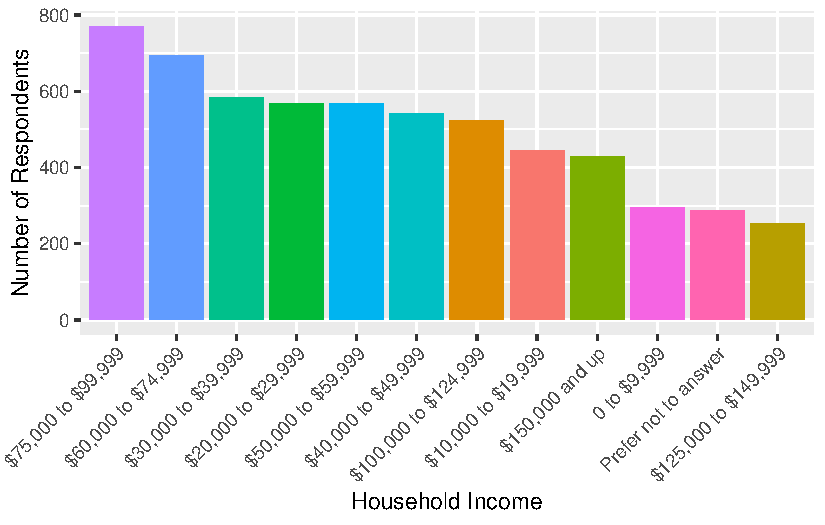
\includegraphics{paper_files/figure-pdf/fig-figure1-1.pdf}

}

\caption{\label{fig-figure1}Distribution of Income from Responses in a
facebook ad}

\end{figure}%

\subsection{Politics Data}\label{sec-pol_data}

Another variable of use is the extent to which the subjects follow
Mr.~Donald Trump, leader of the Republican Party. The possible responses
were `Not at all closely', `Somewhat closely,' `Rather closely' and
`Very Closely,' and the respondents could select one of these options
which will become our measure of measuring subscription to Republican
ideas. This data is represented using a pie chart in
Figure~\ref{fig-figure2}.

\begin{figure}

\centering{

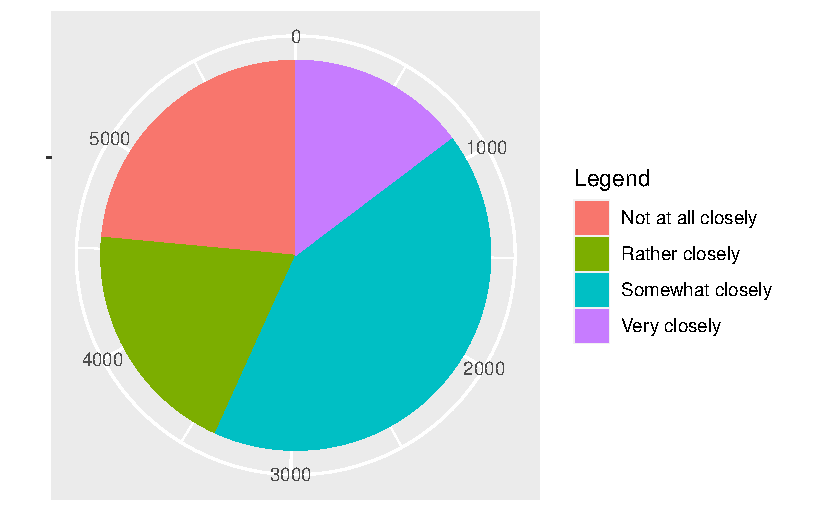
\includegraphics{paper_files/figure-pdf/fig-figure2-1.pdf}

}

\caption{\label{fig-figure2}How Closely People Follow Mr.Donald Trump
from Responses in a facebook ad}

\end{figure}%

\subsection{Ethnicity Data}\label{sec-race_data}

\begin{longtable}[]{@{}lr@{}}

\caption{\label{tbl-race\_dist}Percentage of each Ethnicity from
Responses in a facebook ad}

\tabularnewline

\toprule\noalign{}
Ethnicity & Percentage of Responses \\
\midrule\noalign{}
\endhead
\bottomrule\noalign{}
\endlastfoot
American Indian or Alaskan Native & 0.7554138 \\
Asian or Pacific Islander & 13.5806614 \\
Black or African American & 6.0936713 \\
Hispanic & 8.0577472 \\
Other (please specify) & 2.5851939 \\
White / Caucasian & 68.9273124 \\

\end{longtable}

\section{Results}\label{sec-results}

This papers goal was to identify if lower income household voted against
their own interest. To understand this relationship we used the variable
for how closely a respondent follows Mr.~Donald Trump as our measurement
of subscription to Republican ideas. Using this measurement, we
organized the proportion of individuals by income class to how closely
they follow Mr.~Donald Trump in Figure~\ref{fig-figure3}. This graph
shows that a proportional amount of each income class follows Mr.~Donald
Trump at similar levels across all income levels. Specifically, we mean
the percentage of individuals follow Mr.~Donald Trump at different
levels is the same no matter the income class. This means we can not
conclude that income class impacts how closely individuals follow
Mr.~Donald Trump, and therefor, cannot conclude that different income
levels subscribe to republican ideas more than the other.

\begin{figure}

\centering{

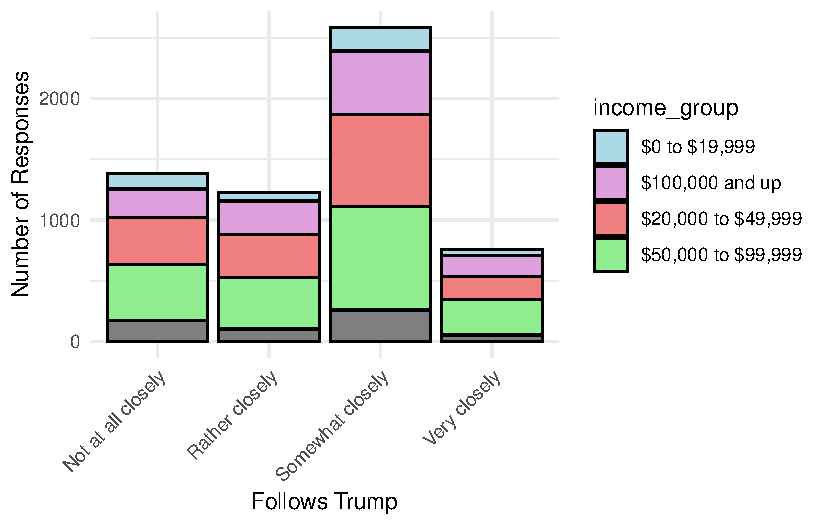
\includegraphics{paper_files/figure-pdf/fig-figure3-1.pdf}

}

\caption{\label{fig-figure3}Number of Respondents who follow Donald
Trump at different levels by Household Income}

\end{figure}%

To further our analysis we computed the same graph however organized by
race not income Figure~\ref{fig-figure4}. This resulted in a similar
result as race is proportional between all levels of following
Mr.~Donald Trump. Therefore, consistent across races at to following
republican rhetoric. Again, this means the same percentage of people
that follow Mr.~Donald Trump at different levels is the same for each
race. Obviously, this is more difficult to conclude for minorities as
their representation within the data set is so small as stated in
Section~\ref{sec-race_data}

\begin{figure}

\centering{

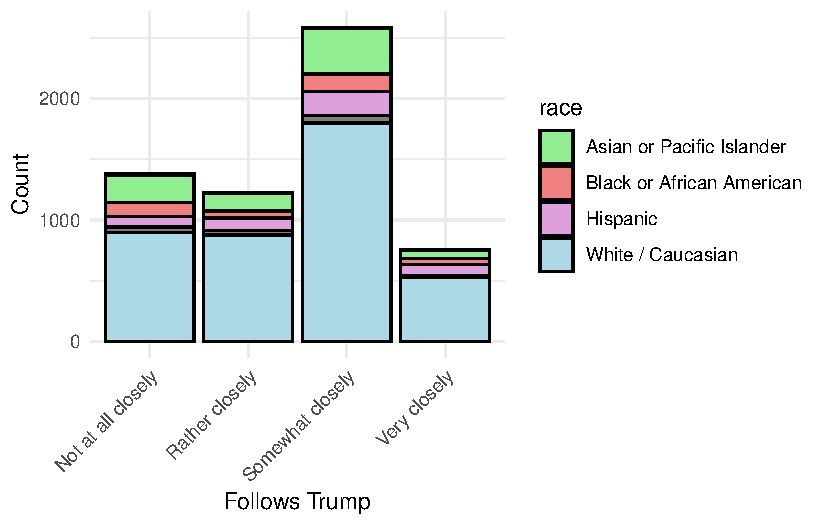
\includegraphics{paper_files/figure-pdf/fig-figure4-1.pdf}

}

\caption{\label{fig-figure4}Number of Respondents who follow Donald
Trump at different levels by Race}

\end{figure}%

Overall, the results of this analysis were inconclusive to measure how
income impacts individuals propensity to follow republican rhetoric.
There are many reasons this could be true and as stated in the
Section~\ref{sec-intro} there are multiple schools of thought previously
studies on the topic.

\newpage

\section*{References}\label{references}
\addcontentsline{toc}{section}{References}

\phantomsection\label{refs}
\begin{CSLReferences}{1}{0}
\bibitem[\citeproctext]{ref-paper}
Allcott, Hunt, Luca Braghieri, Sarah Eichmeyer, and Matthew Gentzkow.
2020. {``The Welfare Effects of Social Media.''} \emph{American Economic
Review}. \url{https://doi.org/10.1257/aer.20190658}.

\bibitem[\citeproctext]{ref-lane}
Gelman, Andrew, Lane Kenworthy, and Yu-Sung Su. 2010. {``Income
Inequality and Partisan Voting in the United States.''} \emph{Social
Science Quarterly}. {[}University of Texas Press, Wiley{]}.
\url{http://www.jstor.org/stable/42956457}.

\bibitem[\citeproctext]{ref-Madrick_2020}
Madrick, Jeff. 2020. {``Why the Working Class Votes Against Its Economic
Interests.''} \emph{The New York Times}, July.
\url{https://www.nytimes.com/2020/07/31/books/review/the-system-robert-reich-break-em-up-zephyr-teachout.html}.

\bibitem[\citeproctext]{ref-her}
Müller, Kirill. 2020. {``Here: A Simpler Way to Find Your Files.''}
\url{https://CRAN.R-project.org/package=here}.

\bibitem[\citeproctext]{ref-citeR}
R Core Team. 2022. \emph{R: A Language and Environment for Statistical
Computing}. Vienna, Austria: R Foundation for Statistical Computing.
\url{https://www.R-project.org/}.

\bibitem[\citeproctext]{ref-hhld}
SCOTT, MICHELLE P. 2024. {``Household Income.''} investopedia.
\url{https://www.investopedia.com/terms/h/household_income.asp}.

\bibitem[\citeproctext]{ref-tidy}
Wickham, Hadley, Mara Averick, Jennifer Bryan, Winston Chang, Lucy
D'Agostino McGowan, Romain François, Garrett Grolemund, et al. 2019.
{``Welcome to the {tidyverse}.''} \emph{Journal of Open Source
Software}. \url{https://doi.org/10.21105/joss.01686}.

\bibitem[\citeproctext]{ref-knitr}
Xie, Yihui. 2023. {``Knitr: A General-Purpose Package for Dynamic Report
Generation in r.''} \url{https://yihui.org/knitr/}.

\end{CSLReferences}



\end{document}
